\nomenclature[]{HMM}{Hidden Markov Model}
\note{Add italics in places}
%\note{Could discuss:
%\\Background:
%What HMMs are,
%why they're useful in AI,
%the different commonly used HMMs. 
%\\ Use in my research:
%How the problem can naturally be described by a HMM,
%Lead into discussion of how DBN is a more natural way to describe the problem and how it leads to efficient factorization of densities for state estimation}
     
HMMs appear frequently in AI literature as they provide an abstract framework to deal with stochastic processes, which themselves are pervasive in their use as a tool to model real-world phenomena. This chapter will outline what HMMs are and their use in literature describing target localization algorithms. A general overview of HMMs can be found in \cite{Murphy1994DynamicLearning}, \cite{Ghahramani2001ANNETWORKS} and \cite{papoulis02}, on which we base the following discussion.

\subsubsection{Markov Processes}\label{subsubsec:MarkovProcesses}
It is instructive to understand what is meant by a stochastic process for some of the concepts mentioned in this thesis. A random process can be described as a family of random variables indexed by a set $\tau$: $\{X_t\}_{t\in\tau}$. Commonly in AI, stochastic processes model the evolution of a random system through \textit{discrete} time steps: $\tau$=$\mathbb N$. Common phenomena modelled by stochastic processes include the growth of a bacterial population and the movement of a gas molecule.\par

A first-order discrete-time Markov process is a stochastic process that describes a system which is in a given state at each time step, with the state changing randomly between steps. The steps are elements of the natural numbers and the random process is a mapping from the natural numbers to states. First-order Markov processes have the additional property that the probability distribution of the n$_{th}$ random variable in the process is conditionally independent of all previous probability distributions in the sequence but the $n-1_{st}$: $P(X_t = x_t | X_{t-1} = x_{t-1}, X_{t-2} = x_{t-2}, ... , X_{1} = x_{1}) = P(X_t = x_t | X_{t-1} = x_{t-1})$. This is often referred to as the Markov Property or the memoryless property of Markov processes. In order to describe a Markov process, it is therefore necessary to describe what is known as the transition function between each pair of timesteps: $P(X_t = x_t | X_{t-1} = x_{t-1})$. A common assumption is that the rules that govern state transitions are time invariant, meaning that they can be specified generally for any given pair of timesteps. This assumption will be made for the subsequent discussion. If $X_t$ is a discrete random variable defined over $S$ states, the transition function can be described by a stochastic matrix T, where T$_{i,j}$ = $P(X_t = j | X_{t-1} = i)$: 

\begin{center}
{$\displaystyle \left({\begin{matrix}T_{1,1}&T_{1,2}&\dots &T_{1,j}&\dots &T_{1,S}\\T_{2,1}&T_{2,2}&\dots &T_{2,j}&\dots &T_{2,S}\\\vdots &\vdots &\ddots &\vdots &\ddots &\vdots \\T_{i,1}&T_{i,2}&\dots &T_{i,j}&\dots &T_{i,S}\\\vdots &\vdots &\ddots &\vdots &\ddots &\vdots \\T_{S,1}&T_{S,2}&\dots &T_{S,j}&\dots &T_{S,S}\\\end{matrix}}\right)$}
\end{center}
\par

Some obvious results are worth pointing out; as for any stochastic matrix, by the axioms of probability theory, the sum of conditional probabilities across {$\displaystyle \sum _{j=1}^{S}T_{i,j}=1$} and the transition probabilities over $k$ timesteps can be described by the $k_{th}$ power of the transition matrix: ${(T^k)}_{i,j}$ = $P(X_{t+k} = j | X_{t} = i)$. Markov processes are often described by graphical models, for example Figure \ref{fig:markov-processes}.
\begin{figure}[b!]
    \centering
    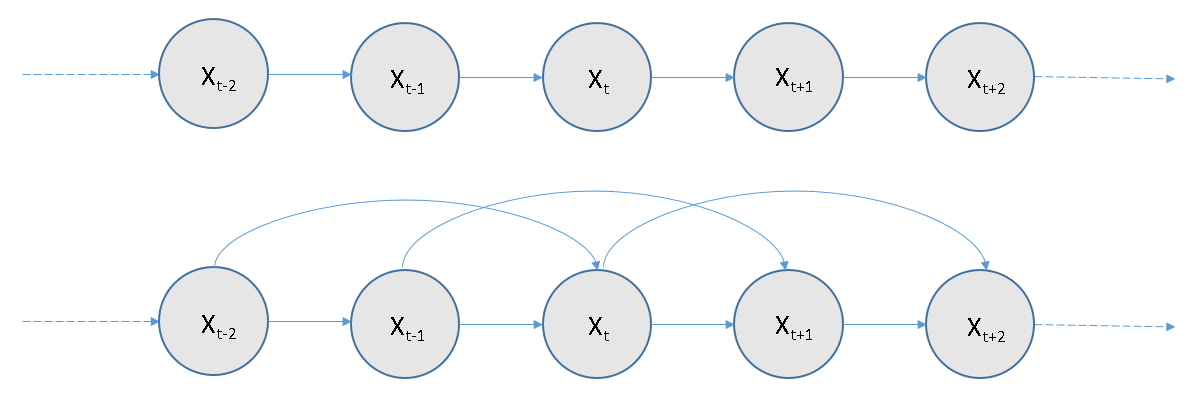
\includegraphics[width=0.8\linewidth]{Chapters/BackgroundKnowledgeAndRelatedWork/MultiAgentTargetDetectionBackground/Figs/MarkovProcesses/MarkovProcesses.png}
    \caption{First and second order Markov processes \cite{AIAMA}}
    \label{fig:markov-processes}
\end{figure}
It also is possible to calculate the probability of the process experiencing a sequence of states from timesteps 1 as far as $t$, using the chain rule of probability and the Markov property:
$P(X_{1:t}) = P(X_1, X_2, ..., X_t) = P(X_1)\times P(X_2 | X_1)\times P(X_3 | X_2, X_1) \times P(X_t | X_{t-1}, X_{t-2}, ... , X_1) = P(X_1) \times \prod_{i=2}^{t}{P(X_i | x_{i-1})}$. Marginalization over variables in this sequence allows the calculation of many useful quantities.
\par

\subsubsection{HMM Description}\label{subsubsec:HMMDesc}
Hidden Markov Models (HMMs) are models that build on the Markov Process model, which describe the evolution of a random system in the language of probability theory. HMMs assume that the system being modeled can be described by a Markov process, but that the states of this process are unobservable. This means that it is not possible to determine the state of the system exactly at any given point in time. However, it is possible to make an observation of a random variable that is related to the hidden state which yields information about the hidden state. A graphical representation of a HMM is shown in figure \ref{fig:hmm}
\begin{figure}[]
    \centering
    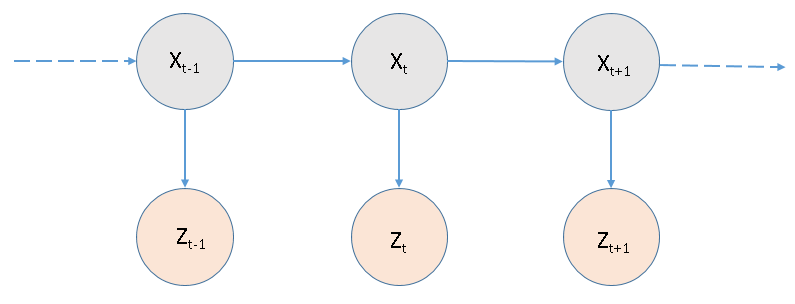
\includegraphics[width=0.8\linewidth]{Chapters/BackgroundKnowledgeAndRelatedWork/MultiAgentTargetDetectionBackground/Figs/HMMs/HMMObservationsOnly.png}
    \caption{A visualisation of a HMM \cite{AIAMA}}
    \label{fig:hmm}
\end{figure}
, where the Markov Process is shown by the variables $X_i$ and the observation variables are shown by variables $E_i$. A HMM can be specified by a triple, $\lambda$ = $(T, O, \pi)$, where $T$ is the stochastic transition matrix, $\pi$ is the initial distribution $P(X_1)$ and O describes the conditional probability of an observation given that the system is in a certain state: $O(E_i, X_i) = P(E_{i} | X_{i})$. Taken together, it is then possible to specify the joint distribution of the hidden state variables and the evidence variables, analogous to the Markov Process: 
$
P(X_{1:t}, E_{1:t}) = P(X_1, X_2, ..., X_t, E_1, E_2, ..., E_t) = P(X_1) \times P(E_1 | X_1) \times
\prod_{i=2}^{t}{(P(X_i | x_{i-1}) \times P(E_t | X_t))}.
$Given this representation, it is then possible to answer questions such as:
\begin{itemize}

    \item Given the HMM, $\lambda$, determine the probability of occurrence of a particular observation sequence, $P(E_{1:t} | \lambda)$
    
    \item Given a sequence of observations $(E_1, E_2, ..., E_n)$, what is the most likely sequence of hidden states that led to these observations? i.e. find \[\argmax_{X_{1:t}} P(X_{1:t} | E_{1:t})\]
    
    \item Determine the parameters of $T$ and $O$, given a training set of observations, i.e. find the solution to \[\argmax_{\lambda} P(E_{1:t} | \lambda)\]
    
    \item \textit{Filtering}: What is the current distribution of the hidden state given all previous evidence ('belief state') of the agent at time t: $P(X_t | E_{1:t})$?
    
    \item \textit{Prediction}: What is the distribution of the hidden state in the future, given all evidence to date: $P(X_{t+k} | E_{1:t})$, for some k$>$0?
    
    \item \textit{Smoothing}: What is the distribution of a past state given all observations up to the current point in time: $P(X_k | E_{1:t})$, for some 0 $\leq$ k $<$ t?
    
\end{itemize}
\par

%Might include a subsection on a taxonomy of commonly used HMMs.

%\subsubsection{Summary}\label{subsubsec:Summary}
%In summary, HMMs can be used to abstractly describe the evolution of a stochastic system. They have been used to achieve state of the art performance in problems such as speech recognition \cite{ChiuSTATE-OF-THE-ARTMODELS} and ... . An comprehensive overview of extensions to the vanilla HMM can be found at \cite{Murphy1994DynamicLearning}.